%&pdflatex
\documentclass[11pt,onecolumn]{scrartcl}
\usepackage[utf8]{inputenc}
\usepackage{amsmath,amssymb,amsfonts,mathrsfs,amsthm}
\usepackage[top=2cm,bottom=3cm,left=2.5cm,right=2cm]{geometry}
\usepackage{amssymb}
\usepackage{amscd}
\usepackage{listings}
\usepackage{array}
\usepackage{mathtools}
\usepackage{dsfont}
\usepackage{graphicx}
\usepackage{pdfpages}
\usepackage[textsize=footnotesize,color=green]{todonotes}
\usepackage{algorithm, algorithmic}
\usepackage{array}
\usepackage{bm}
\usepackage{tikz}
\usepackage{subfigure}
\usepackage[normalem]{ulem}

\newcommand{\bs}[1]{\boldsymbol{#1}}
\DeclareMathOperator{\diag}{diag}

\newcommand{\equaldef}{\stackrel{\mathrm{def}}{=}}

\newcommand{\tablab}[1]{\label{tab:#1}}
\newcommand{\tabref}[1]{Table~\ref{tab:#1}}

\newcommand{\theolab}[1]{\label{theo:#1}}
\newcommand{\theoref}[1]{\ref{theo:#1}}
\newcommand{\eqnlab}[1]{\label{eq:#1}}
\newcommand{\eqnref}[1]{\eqref{eq:#1}}
\newcommand{\seclab}[1]{\label{sec:#1}}
\newcommand{\secref}[1]{\ref{sec:#1}}
\newcommand{\lemlab}[1]{\label{lem:#1}}
\newcommand{\lemref}[1]{\ref{lem:#1}}

\newcommand{\mb}[1]{\mathbf{#1}}
\newcommand{\mbb}[1]{\mathbb{#1}}
\newcommand{\mc}[1]{\mathcal{#1}}
\newcommand{\nor}[1]{\left\| #1 \right\|}
\newcommand{\snor}[1]{\left| #1 \right|}
\newcommand{\LRp}[1]{\left( #1 \right)}
\newcommand{\LRs}[1]{\left[ #1 \right]}
\newcommand{\LRa}[1]{\left\langle #1 \right\rangle}
\newcommand{\LRc}[1]{\left\{ #1 \right\}}
\newcommand{\LRb}[1]{\left| #1 \right|}

\newcommand{\tanbui}[2]{\textcolor{blue}{\sout{#1}} \textcolor{red}{#2}}
\newcommand{\Grad} {\ensuremath{\nabla}}
\newcommand{\Div} {\ensuremath{\nabla\cdot}}
\newcommand{\Nel} {\ensuremath{{N^\text{el}}}}
\newcommand{\jump}[1] {\ensuremath{\LRs{\!\left[#1\right]\!}}}
\newcommand{\uh}{\widehat{u}}
\newcommand{\fnh}{\widehat{f}_n}
\renewcommand{\L}{L^2\LRp{\Omega}}
\newcommand{\pO}{\partial\Omega}
\newcommand{\Gh}{\Gamma_h}
\newcommand{\Gm}{\Gamma_{-}}
\newcommand{\Gp}{\Gamma_{+}}
\newcommand{\Go}{\Gamma_0}
\newcommand{\Oh}{\Omega_h}

\newcommand{\eval}[2][\right]{\relax
  \ifx#1\right\relax \left.\fi#2#1\rvert}

\def\etal{{\it et al.~}}

\newcommand{\vect}[1]{\ensuremath\boldsymbol{#1}}
\newcommand{\tensor}[1]{\underline{\vect{#1}}}
\newcommand{\del}{\Delta}
\newcommand{\grad}{\nabla}
\newcommand{\curl}{\grad \times}
\renewcommand{\div}{\grad \cdot}
\newcommand{\ip}[1]{\left\langle #1 \right\rangle}
\newcommand{\eip}[1]{a\left( #1 \right)}
\newcommand{\pd}[2]{\frac{\partial#1}{\partial#2}}
\newcommand{\pdd}[2]{\frac{\partial^2#1}{\partial#2^2}}

\newcommand{\circone}{\ding{192}}
\newcommand{\circtwo}{\ding{193}}
\newcommand{\circthree}{\ding{194}}
\newcommand{\circfour}{\ding{195}}
\newcommand{\circfive}{\ding{196}}

\def\arr#1#2#3#4{\left[
\begin{array}{cc}
#1 & #2\\
#3 & #4\\
\end{array}
\right]}
\def\vecttwo#1#2{\left[
\begin{array}{c}
#1\\
#2\\
\end{array}
\right]}
\def\vectthree#1#2#3{\left[
\begin{array}{c}
#1\\
#2\\
#3\\
\end{array}
\right]}
\def\vectfour#1#2#3#4{\left[
\begin{array}{c}
#1\\
#2\\
#3\\
#4\\
\end{array}
\right]}

\newtheorem{proposition}{Proposition}
\newtheorem{corollary}{Corollary}
\newtheorem{theorem}{Theorem}
\newtheorem{lemma}{Lemma}

\newcommand{\G} {\Gamma}
\newcommand{\Gin} {\Gamma_{in}}
\newcommand{\Gout} {\Gamma_{out}}

\newtheorem{remark}{Remark}

%\title{$\epsilon$-explicit analysis of DPG for convection-dominated diffusion}
\title{Notes on the solution of the Navier-Stokes equations using DPG}
\date{}
\begin{document}

\maketitle

\section{Linearized Navier-Stokes equations}

Our approach in applying DPG to the Navier-Stokes equations is to linearize, and then extrapolate DPG to the linearized equations.  The Navier-Stokes equations can be written in terms of the Euler variables $U$ and viscous stresses $\Sigma$ as
\begin{align*}
\div\LRp{F(U)-G(U,\Sigma)}&=0\\
E\Sigma - \grad U&=0.
\end{align*}
The linearized Navier-Stokes equations can be written
\begin{align*}
\div\LRp{\LRp{F_{,U}(U)-G_{,U}(U,\Sigma)}dU-G_{,\Sigma}(U,\Sigma)d\Sigma}&=\text{conservation law residual}\\
E\Sigma - \grad U&= \text{stress law residual}.
\end{align*}
We test the conservation laws with test functions $V$ and stress laws with test functions $V$.  The test norm is extrapolated by identifying like terms with convection-diffusion and extrapolating test norms for groups of variables
\begin{align*}
\nor{\LRp{V,W}}_V^2 =& \nor{V}^2+ \nor{\LRp{F_{,U}(U)-G_{,U}(U,\Sigma)}^TV}^2 + \frac{1}{\rm Re}\nor{G_{,\Sigma}(U,\Sigma)^T\grad V}^2 \\
&+ \min\LRc{{\rm Re},\frac{1}{\LRb{K}}}\nor{W}^2 + \nor{\div W}^2
\end{align*}

\section{Conditioning of local problems}

Notice that, under the above test norm, $V$ and $W$ are decoupled.  Likewise, our local problem decouples into three local problems with submatrices $A_1, A_2, A_3$, where $A_1$ is $\tau_1$ and $\tau_2$, coupled together by the stress equation.  $A_2$ has to do with $\tau_3$, which is decoupled from $\tau_1,\tau_2$ by merit that temperature $T$ and heat flux $q$ do not show up in the stress equations.  $A_3$ is related to $v_1,\ldots, v_4$, and is the main cause of conditioning problems.  

\begin{figure}[!h]
\centering
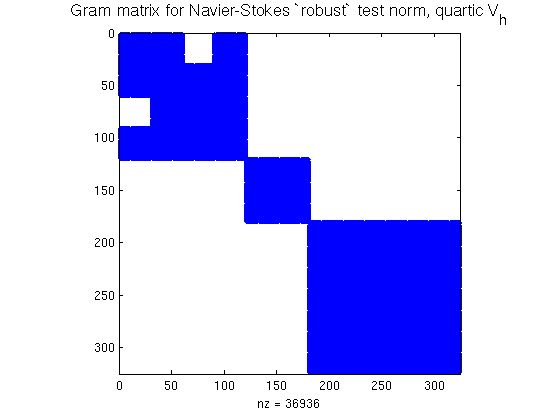
\includegraphics[scale=.75]{figs/GramMatrixSpy.png}
%\subfigure[$\alpha = 1$]{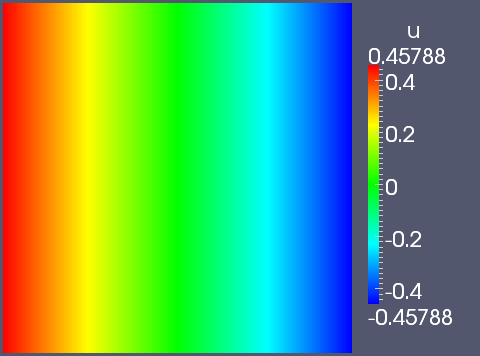
\includegraphics[scale=.475]{figs/aOneConstant.png}}
\caption{Spy plot of the Riesz operator under the robust test norm for Navier-Stokes.}
\end{figure}

We use ${\rm Re} = 100$ to eliminate robustness issues.  After 7 refinements, we have $h_{\rm min} \approx .002$.  The magnitude of the $\L$ term on $v$ is proportional to $dt^{-1}$, and with $dt = .1$, we have a condition number of $\kappa(A_3) = O(1e8)$.  

\begin{figure}[!h]
\centering
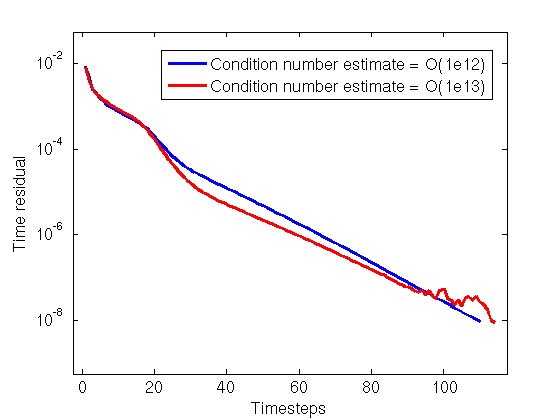
\includegraphics[scale=.8]{figs/NSConditionNumbers.png}
\caption{Transient residual behavior under poor conditioning.  The condition number estimate is for the entire system; the individual decoupled blocks have significantly lower condition number estimates.}
\end{figure}

Our condition number is now of the order of single precision arithmetic, and we begin to see either divergence or non-monotonic convergence of the transient residual.  Since condition numbers can be misleading, we computed a discrete residual for 100 random loads and averaged them to confirm that the error in our approximation is indeed $O(\kappa(A_3))$.  

\begin{figure}[!h]
\centering
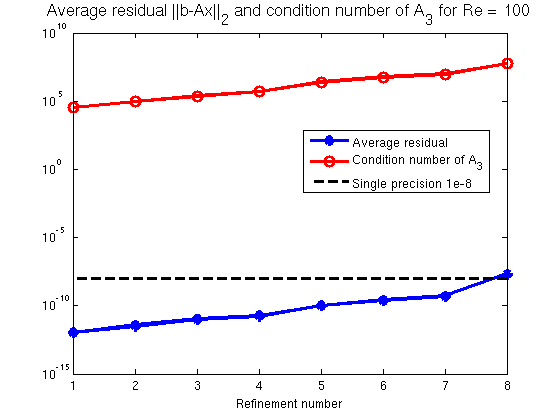
\includegraphics[scale=.8]{figs/NSResidualCondition.png}
\caption{Average discrete residual $\nor{b-Ax}_2$.  Convergence of the pseudo-time iteration stalls after the 8th refinement step due to conditioning issues.}
\end{figure}

\subsection{ Cholesky stability}

We found that Cholesky decompositions of the matrices led to factorizations with more diagonally dominant terms when compared to LU factorizations.  Additionally, the failure of Cholesky due to numerical indefiniteness signals a clear stopping point for the method due to roundoff effects.  

\section{Singularity in $\rho$}

The singularity in $\rho$ at the plate edge is independent of the Reynolds number and appears to be unbounded.  For $Re = 100$, the singularity continues to grow in magnitude despite the mesh having resolved the diffusive length scale.  

\section{Solution strategy}

Specify parameters and motivation, pseudo-time step and inner Newton iteration.  

\subsection{Nested solves}

For the compressible Navier-Stokes equations, density $\rho$ and temperature $T$ must both be guaranteed positive to have a physically realistic solution.  Numerically, non-positivity of $\rho$ and $T$ can cause non-convergence of our nonlinear iteration, and in some cases, solution blowup.  In order to ensure positivity of $\rho$ and $T$ for these simulations, during each timestep, we apply a Newton-Raphson with line search to ensure that 
\begin{align*}
\rho + \triangle \rho &> 0\\
T + \triangle T &> 0,
\end{align*}
where $\triangle \rho$ and $\triangle T$ are the Newton-Raphson updates to the solution at each step.  In similar applications, multiple Newton steps per timestep have been shown to accelerate convergence of the pseudo-time algorithm \cite{kirkThesis}.  

\subsection{Adaptive time tolerance}

A common technique in the solution of the steady-state Navier-Stokes equations under implicit time discretizations is the use of variable time-stepping.  Typically, these schemes can be expressed as such: at a timestep $i$, the next time step can be expressed as a scaling of the timestep $k$ steps ago
\[
dt_{i+1} = dt_{i-k} \LRp{\frac{R_{i-k}}{R_i}}^r,
\]
where $R_{i-k}$ and $R_i$ are the transient residuals at the $i$th and $(i-k)$th timesteps.  The intuition behind this algorithm is that as transient behavior dies out, we can take larger and larger timesteps, thus accelerating our convergence to steady state.  

\textcolor{red}{Talk about DPG and ``changing targets" with variable timestep.}

\bibliographystyle{plain}
\bibliography{paper}


\end{document}
